\chapter[Introdução]{Introdução}

Com continuo crescimento do e-commerce no Brasil nos últimos anos e a adesão cada vez maior de novas lojas no Marketplace, traz consigo um aumento considerável na entrada de novos produtos no site da companhia. Tal confirmação pode ser observado na \autoref{quantidade_de_produtos_por_mes}.

\begin{figure}[htb]
	\caption{\label{quantidade_de_produtos_por_mes} Quantidade de Produtos ao longo dos Meses 2018+}
	\begin{center}
	    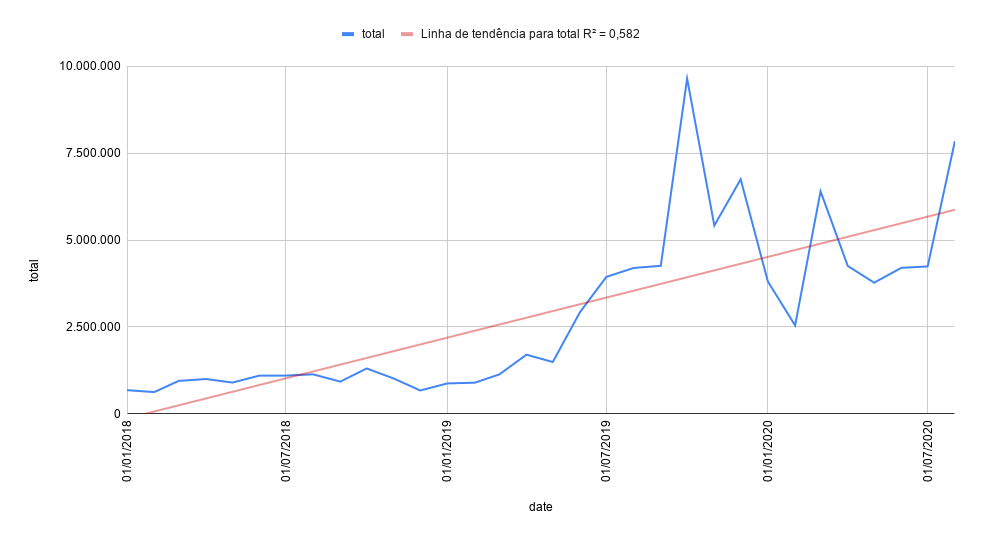
\includegraphics[width=\textwidth]{artigo/recursos/imagens/Quantidade de Produtos ao longo dos Meses 2018+.png}
	\end{center}
	\legend{Fonte: Elaborado pelo Autor}
\end{figure}

Neste contexto a B2W possui milhares de categorias para a classificação individual de produtos, como pode ser visto na tabela \autoref{tab:quantidade_de_categorias}, essa quantidade de categorias gera muita confusão e erros na hora de fazer a classificação dos produtos pelas lojas (sellers).

\begin{table}[]
    \centering
    \caption{Quantidade de Categorias}
    \begin{tabular}{r|l} \hline
        Departamento & 60  \\ \hline
        Setor & 1152 \\ \hline
        Família & 4595 \\ \hline
        Subfamília & 8885 \\ \hline
    \end{tabular}
    \legend{Fonte: Elaborado pelo Autor}
    \label{tab:quantidade_de_categorias}
\end{table}

Portanto, se faz necessário a criação de um sistema capaz de fazer esta categorização de forma automática a fim de reduzir o custo, tempo e elevar a assertividade da classificação de produtos na entrada de novos itens no marketplace. 

Para a resolução deste problema, foi desenvolvido uma arquitetura de Redes Neurais Artificiais utilizando dados heterogêneos não estruturados (texto e imagem) dos produtos a fim de tornar a classificação mais eficiente do ponto de vista de assertividade.

\section{PORQUE UTILIZAR TEXTO E IMAGEM}

A necessidade de utilizar dois tipos de dados tão distintos durante a classificação, se faz necessário devido em alguns casos esses dados individualmente não possuírem informação o suficiente para classificar adequadamente a categoria do produto. Pode ser visto um exemplo de ambiguidade de produtos na \autoref{produtos_similares} em categorias distintas.

\begin{figure}[htb]
	\caption{\label{produtos_similares} Produtos similares em categorias distintas}
	\begin{center}
	    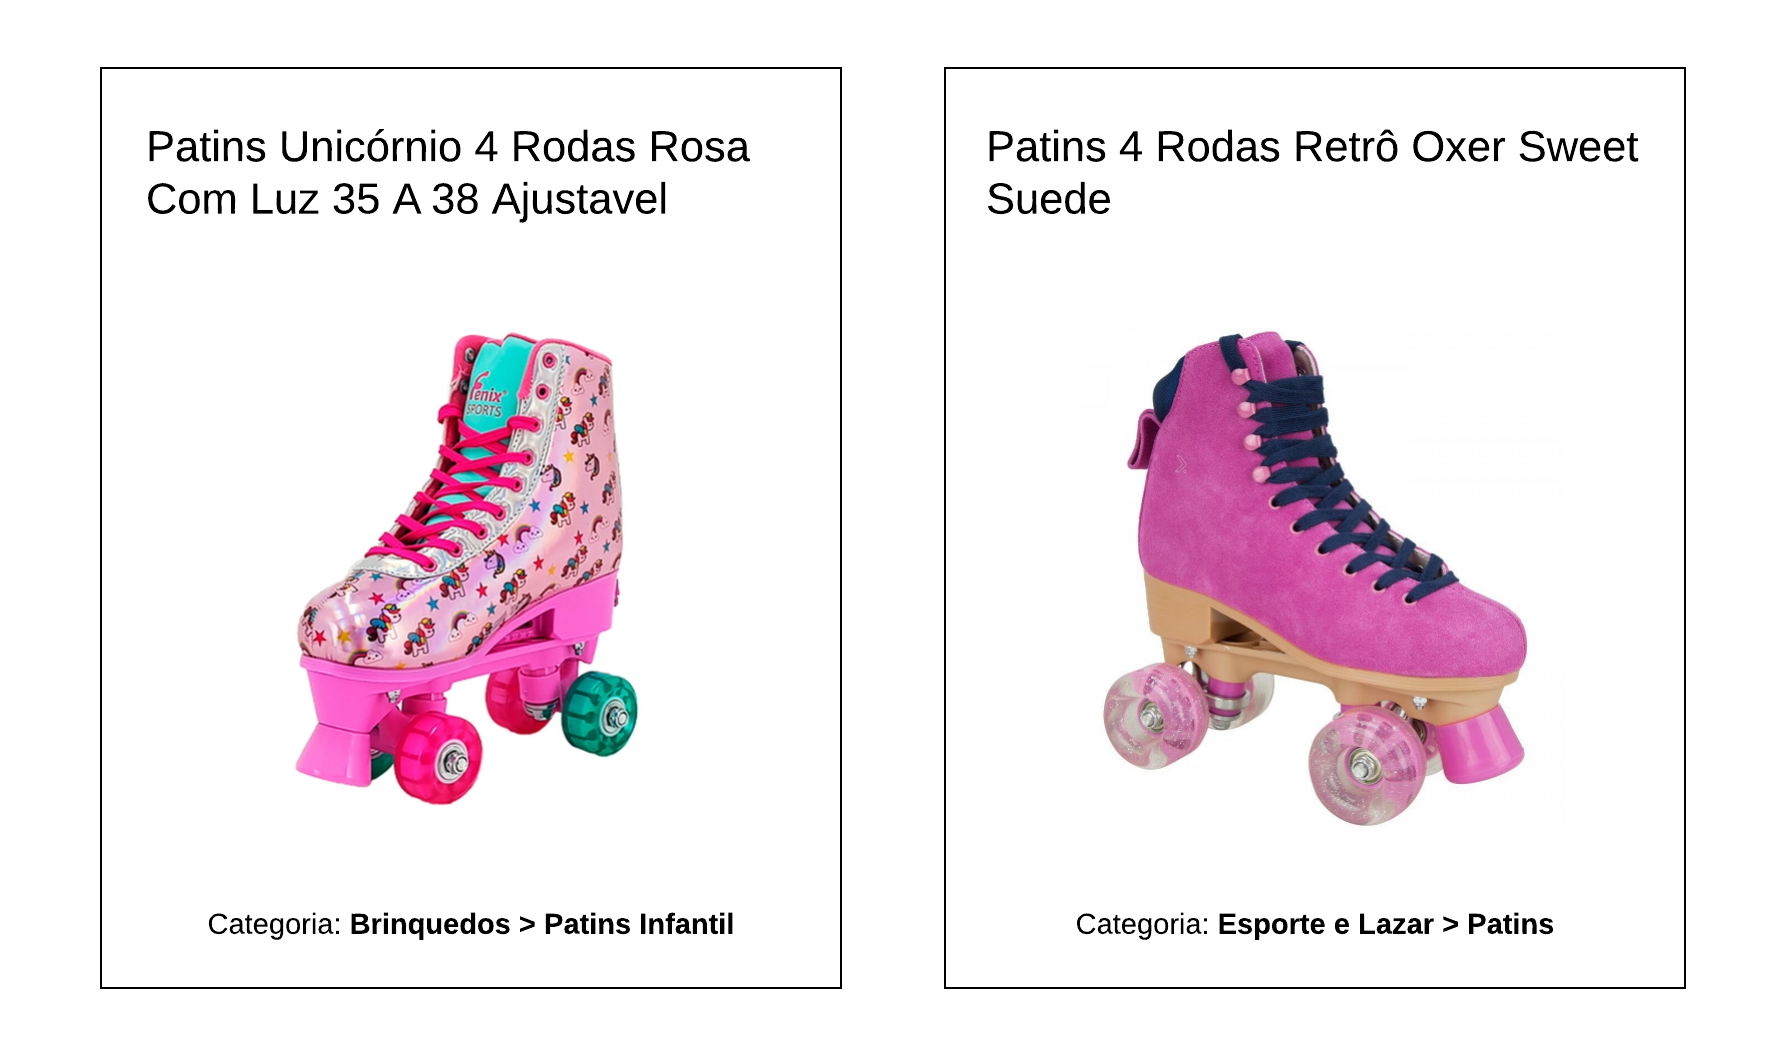
\includegraphics[scale=0.5]{artigo/recursos/imagens/produtos-similares.png}
	\end{center}
	\legend{Fonte: Elaborado pelo Autor}
\end{figure}

\section{ESTRUTURA DAS CATEGORIAS}

A estrutura das categorias é em formato de árvore e pode ser visto na \autoref{arvore_de_categorias}, onde os níveis superiores são mais genéricos e conforme os níveis mais baixos, esses são se especificando cada vez mais. Hoje existe um conjunto total de X categorias.

\begin{figure}[htb]
	\caption{\label{arvore_de_categorias} Estrutura das categorias em árvore}
	\begin{center}
	    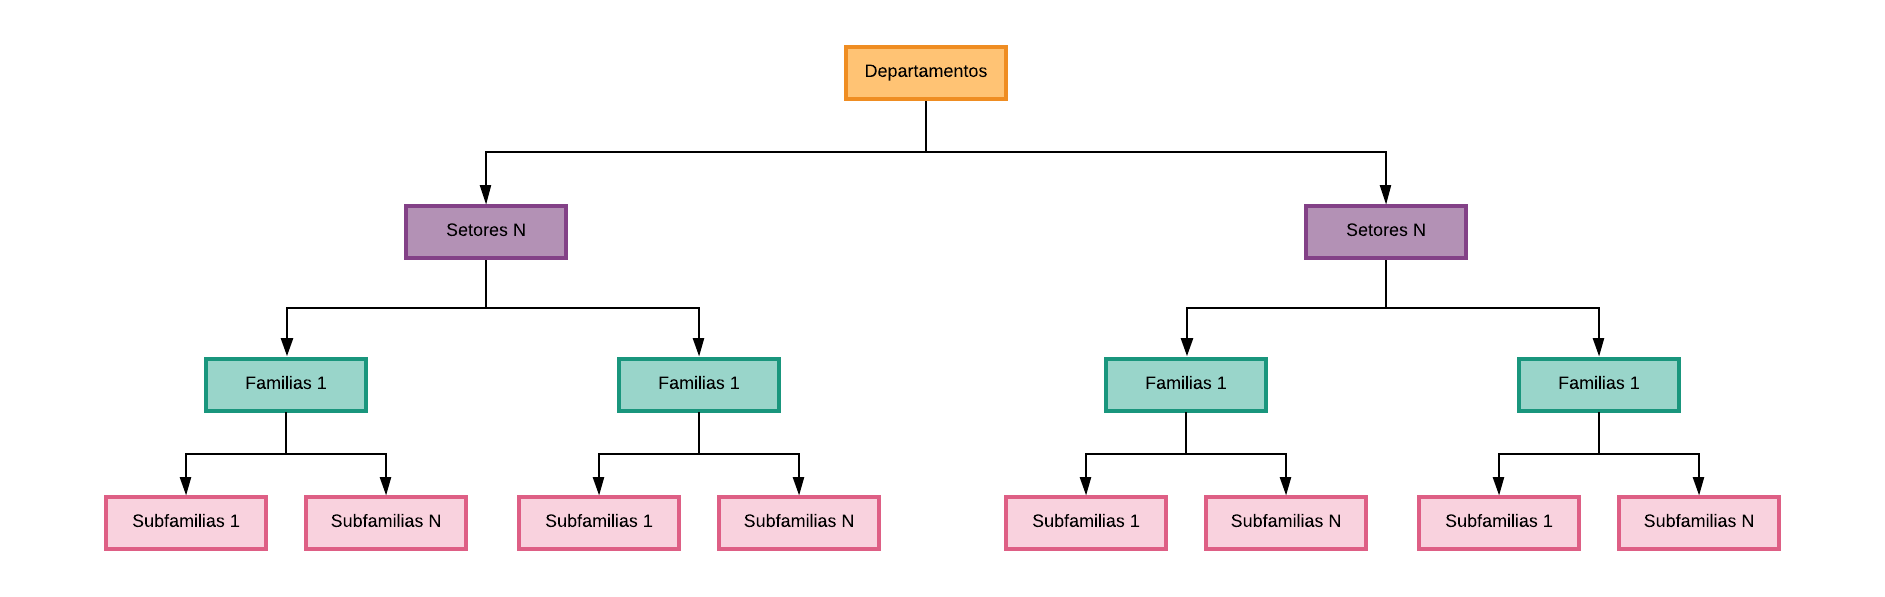
\includegraphics[scale=0.5]{artigo/recursos/imagens/arvore-de-categorias.png}
	\end{center}
	\legend{Fonte: Elaborado pelo Autor}
\end{figure}

\section{PROBLEMAS NOS DADOS}

Como todo conjunto de dados do mundo real, o nosso conjunto de dados não é diferente e possui diversos problemas. Ambiguidades de Categorias, Ruídos e desbalanceamento. A seguir, será feito um resumo dos principais problemas e dificuldades encontrados.

\subsection{AMBIGUIDADES}

A ambiguidade de categorias é outro problema encontrado no nosso conjunto dados, isso de deve a criação desordenada e descentralizada de categorias ao longo dos anos para atender diversos setores da companhia com objetivos distintos. 

\begin{table}[h]
    \centering
    \caption{Amostra de categorias ambíguas no contexto de Mouse para computador}
    \tiny
    \begin{tabularx}{\textwidth}{X|X|X|X} 
        \textbf{DEPARTAMENTO} & \textbf{SETOR} & \textbf{FAMÍLIA} & \textbf{SUBFAMÍLIA} \\ \hline
        INFORMÁTICA ACESSÓRIOS & MOUSE & MOUSE COM FIO & MOUSE COM FIO \\ \hline
        INFORMÁTICA ACESSÓRIOS & MOUSE & MOUSE WIRELESS & MOUSE WIRELESS \\ \hline
        INFORMÁTICA ACESSÓRIOS & MOUSE & MOUSE RETRÁTIL & MOUSE RETRÁTIL \\ \hline
        PC GAMER & MOUSE GAMER & MOUSE COM FIO & MOUSE COM FIO \\ \hline
        PC GAMER & MOUSE GAMER & MOUSE WIRELESS & MOUSE WIRELESS \\ \hline
        PC GAMER & COMBO GAMER & TECLADO E MOUSE & TECLADO E MOUSE \\ \hline
        PC GAMER & COMBO GAMER & MOUSE + MOUSEPAD GAMER & MOUSE + MOUSEPAD GAMER
    \end{tabularx}
    \legend{Fonte: Elaborado pelo autor}
    \label{tab:ambiguidades}
\end{table}

\subsection{RUÍDOS NOS DADOS}

Além dos problemas de ambiguidades, há problemas também de produtos mal categorizados anteriormente, onde por algum equívoco (dificuldade/ambiguidade), um produto foi alocado em uma categoria erroneamente.

Podemos citar um exemplo de que um celular, que poderia estar alocado em televisões. Se este item for selecionado para o treinamento, logo fará com que outros celulares sejam classificados como televisão, um outro problema é uma distorção durante a avaliação dos produtos, pois se esse produto foi selecionado para o conjunto de teste do modelo, logo ele seria classificado como celular, mas a categoria atrelada à ele seria a de televisão.

\subsection{DESBALANCEAMENTO NAS CATEGORIAS}

O problema de desbalanceamento de dados também se encontra presente, para mitigar esse problema utilizamos algumas técnicas como: oversampling, undersampling e  uma função de erro especializada para dados desbalanceados.

\begin{figure}[htb]
	\caption{\label{char_bar_produtos_por_categoria} Quantidade de Produtos Por Departamento}
	\begin{center}
	    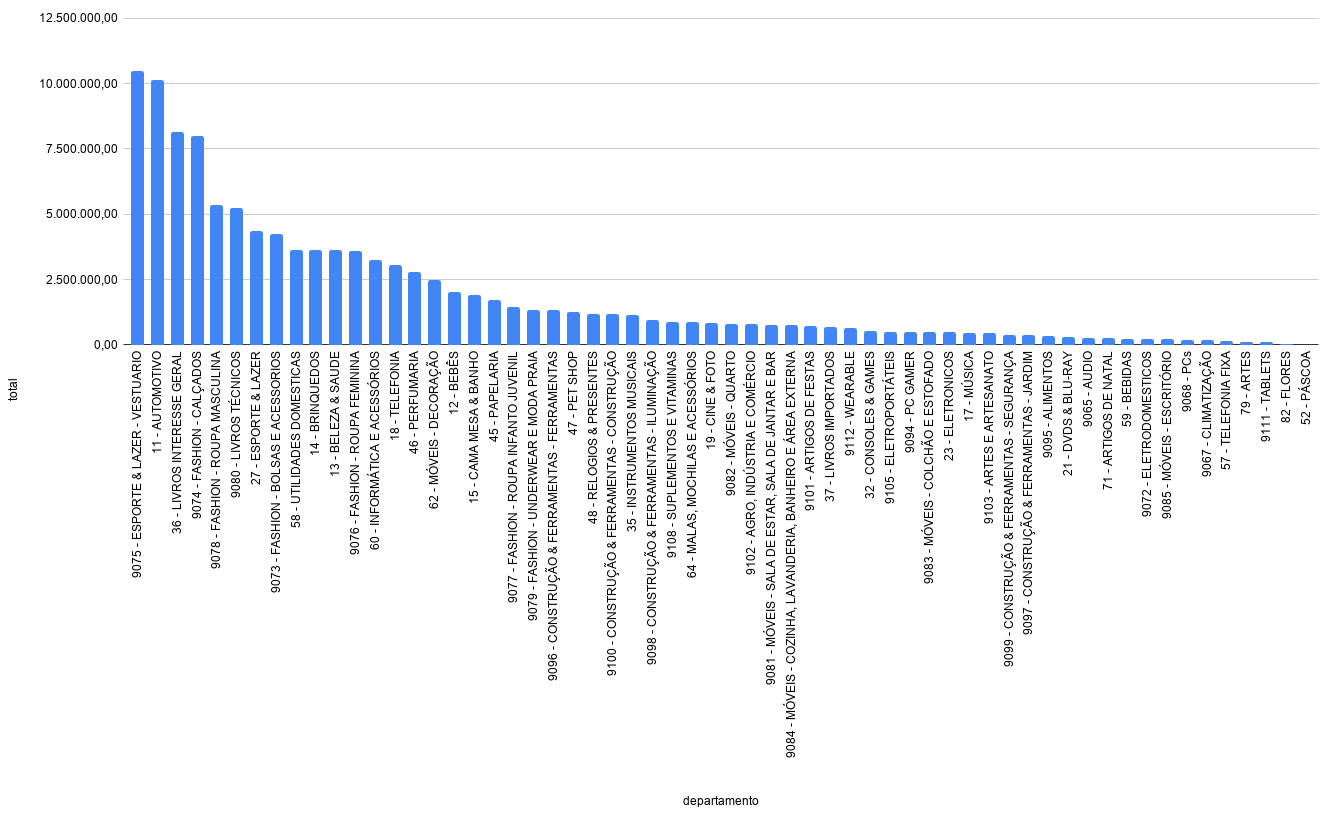
\includegraphics[width=\textwidth]{artigo/recursos/imagens/Quantidade de Produtos por Departamento.png}
	\end{center}
	\legend{Fonte: Elaborado pelo Autor}
\end{figure}

\subsection{LÍNGUA PRÓPRIA}

Os títulos dos produtos são tão distintos nas palavras e na forma de escrever da linguá comum, que partimos do princípio que estamos trabalhando como uma língua distinta de todas as outras. Pois não conseguimos aplicar nenhuma técnica tradicional de Processamento de Linguagem Natural como: lemmantize, stemmer ou mesmo stop-words.

\begin{itemize}
\item Smartphone Samsung Galaxy S10e 128GB Dual Chip Android 9.0 Tela 5,8" Octa-Core 4G Câmera 12MP + 16MP - Preto
\item Geladeira/Refrigerador Electrolux DC35A Branca 260L Cycle Defrost - 220v
\item Tapete Para Sala Shaggy Requinte Casa Dona 100x150cm Cinza
\end{itemize}

É possível observar nos exemplos acima que não seguem nenhuma regra gramatical do português. Além de quê, com a entrada de novos produtos de outros países, presumir regras gramaticais parece imprudente.